\section{Reimplementation Strategy}
\label{sec:remplementation}

The code accompanying the original paper  is poorly written, poorly documented, and is formed of several complex and independant blocks. 
To effectively explore the core contributions of the paper,
we decided to reimplement parts of it with a more focused scope.

In our approach, we focused on reconstructing arm motion from video data,
a simplification that allowed us to tackle the fundamental 
aspects of the methodology without the computational burden of full-body modeling.

Our code is available and documented on~\href{https://github.com/balthazarneveu/monocular_pose_and_forces_estimation}{GitHub}.

\subsection{Overview}
\label{subsec:overview}
Our simplification regarding the original paper are listed below:
\begin{itemize}
    \item Only the arm motion (shoulder, elbow and wrist) is considered and not the full body.
    \subitem - We end up with the arm state $q$ being a quaternion describing 
    the upper arm state and a single elbow angle for the forearm state.
    \subitem - Shoulder is fixed to the world frame.
    \item Do not deal with objects and external contact forces.
    \item Act under controlled conditions.
    \subitem - A correct lighting and a static background to simplify the vision task.
    \subitem - We make sure that the camera is on a tripod and geometrically calibrated.
\end{itemize}

Regarding implementation, we started from scratch. Instead of trying to re-implement
the whole inverse dynamics optimization framework at once, we progressively built a solution.
Since the arm has only 4 degrees of freedom, leading to 3x 3D joints, 
fitting the full camera parameters (extrinsics and intrinsics) at the same time
as fitting the whole arm dynamics is not possible (under determined system).
\begin{itemize}
    \item (\ref{subsec:vision_pipeline}) - Vision pipeline 
    extracts 3x 2D and 3x 3D arm estimated joints positions.
    \item (\ref{subsec:inverse_kinematics}) - We use inverse kinematics  
    on the 3D points to get coarse robot arm state.
    \item (\ref{subsec:cam_estim}) - We fit the camera/shoulder translation 
    by minimizing the 2D reprojection error of the 3D points.
\end{itemize}



% WARNING: !!!!!!!!!!!! 
Due to lack of time, we were not able to implement the inverse kinematics which minimizes jointly
the camera pose and the arm state $q$.

Finally, using the above $q$ state estimation as an initialization,
we implemented a proof of concept for the inverse dynamics optimizer focusing on:
\begin{itemize}
    \item minimizing $l_{\text{3D}}$ the 3D reprojection error of the arm joints.
    \item under relaxed dynamic constraint.
    \item under smooth motion constraints (velocities and accelerations)
\end{itemize}
% WARNING: !!!!!!!!!!!! 


\subsection{Vision Pipeline}
\label{subsec:vision_pipeline}

For 2D and 3D human pose estimation, we utilized the MediaPipe framework~\cite{lugaresi2019mediapipe}, which offers a more modern alternative 
to OpenPose. MediaPipe simplifies the vision pipeline by also replacing HMR in our usecase. An illustration of MediaPipe's inference results 
can be seen in~\cref{fig:mediapipe}. We then only used the arm joint 2D and 3D positions. 

\begin{figure}
    \centering
    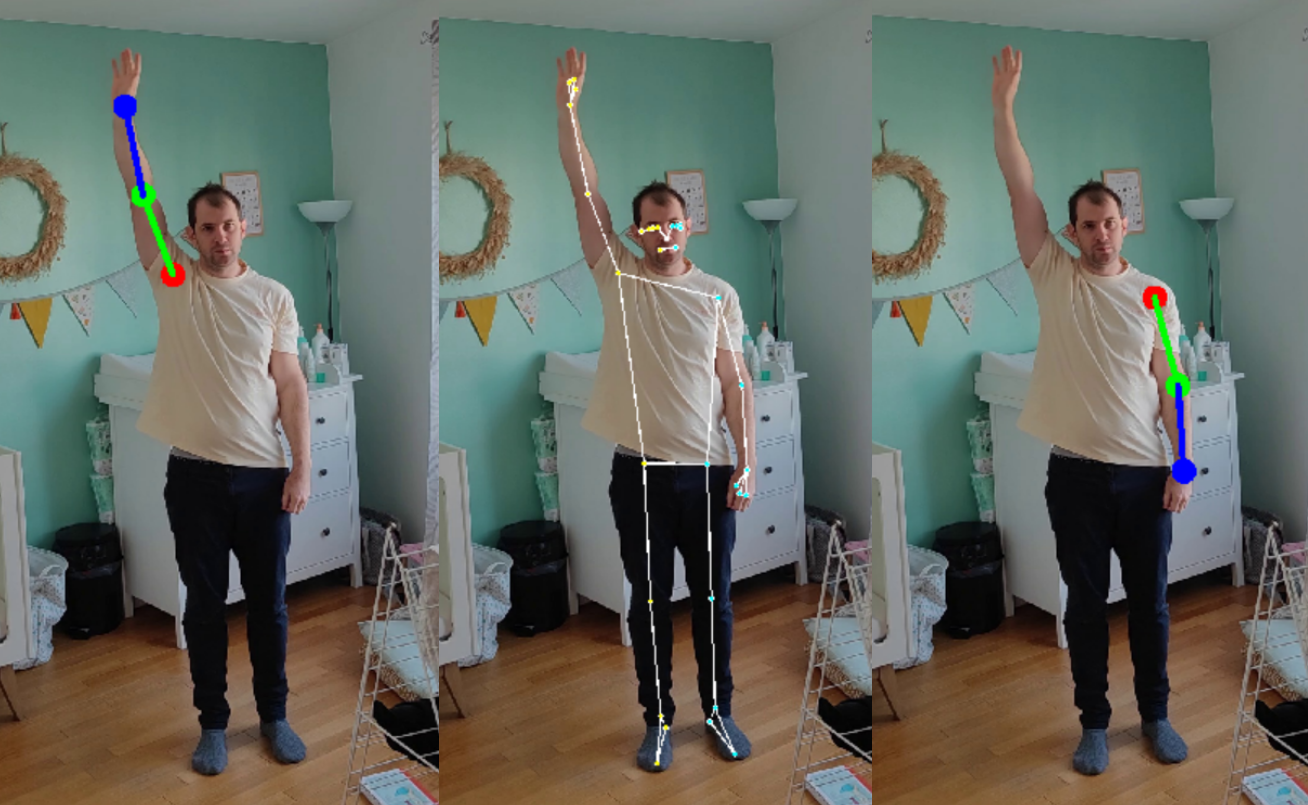
\includegraphics[width=8cm]{figures/pose_detection_mediapipe_collage.png}
    \caption{
    \color{red}Shoulder, \color{darkgreen}elbow, \color{blue}wrist \color{black} joints indicated with dots
    are linked by the \color{darkgreen}upper arm \color{black} and \color{blue}forearm \color{black}. 2D and 3D data is extracted from
    the full body pose estimated with MediaPipe.
    }
    \label{fig:mediapipe}
\end{figure}

Although we experimented with the contact recognizer component, we did not use it into our pipeline since we do not model contact.

\subsection{Arm Model}
\label{subsec:arm_model}
We modelled the arm in Pinocchio~\cite{carpentier2019pinocchio}. The shoulder is represented by a spherical joint, allowing for three degrees 
of freedom. This is expressed as a quaternion in the state vector \(q\). The elbow is represented by a revolute joint, which permits rotation 
within a plane, resulting in a single degree of freedom. The state \(q\) therefore consists of five elements: the first four correspond to the 
shoulder quaternion, and the fifth represents the elbow angle, which is constrained within the range \([0, \pi]\) radians. The dimensions of 
the arm are fixed with the forearm and upper arm lengths fixed at 27 cm and 23 cm, respectively. See~\cref{fig:arm_model}

\begin{figure}
    \centering
    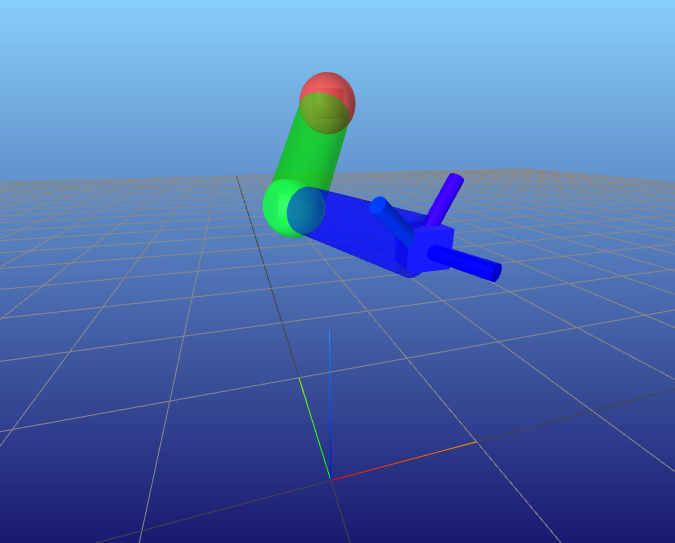
\includegraphics[width=0.3\textwidth]{figures/live_arm.png}
    \caption{Arm Model vizualisation}
    \label{fig:arm_model}
\end{figure}

\subsection{Inverse Kinematics}
\label{subsec:inverse_kinematics}
To get proper initializations to feed to the inverse dynamics optimizer, we relied on the 3D positions of the arm joints estimated by MediaPipe~\cite{lugaresi2019mediapipe}.
From a sequence of 3D positions of the arm joints, we used the inverse kinematics approach to estimate the joint angles.
Inverse kinematics is higly relying on the Pinocchio library ~\cite{carpentier2019pinocchio} to compute 
the Jacobian and perform forward kinematics (compute the 3D positions  $M(t)_{j}$ of the joints from the joint angles $q(t)$).
% @TODO: Add equations for IK with the 2 tasks (elbow and wrist 3D positions)

Devil is in the details, and we had to be careful about the following points while implementing:
\begin{itemize}
    \item We provide 2 tasks to the inverse kinematics solver: one for the elbow 3D position and one for the wrist 3D position. 
    Order matters, elbow comes first.
    \item The mediapipe 3D estimations are not perfect but the most nottable issue is that 
    the upper arm and the forearm lengths are not constant across time. To overcome this limitation,
    3D positions are re-scaled to match the expected nominal model arm length. 
    This arm length normalization ensures that a solution exists but on the other hand, it may introduce reprojection errors.
\end{itemize}
Although nothing grants temporal smoothness of the estimated joint angles, we recursively feed the previous solution as an initial guess to the current timestep.
This simple trick gives good results in practice (assessed qualitatively on the match between the moving arm and the video).


\subsection{Camera position}
\label{subsec:cam_estim}

\noindent\textbf{Problem formulation.} Since the upper arm can rotate in all directions and since we're not using any priors to constrain 
the arm motion (at the shoulder level), moving the camera around the arm is equivalent to spinning the arm around itself. 
Our simplification unfortunately leads to a degenerate problem where the camera rotation may end up being redundant with the arm rotation.
To avoid this issue, we decided to fix the camera orientation. 
We estimate the camera 3D position $P_{\text{cam}}(t)$ 
by jointly minimizing the 2D reprojection error of joints.
$$\underset{P_{\text{cam}}(t)}{min}\sum_{j\in{\text{shoulder, elbow, wrist}}} ||K.\big[Q_{\text{cam}} | P_{\text{cam}}(t)] \vec{X}^{(j)}(t) - \vec{x}^{(j)}(t) ||$$
where
\begin{itemize}
    \item $K$ is the camera 3x3 intrinsic matrix
    \item $Q$ is the camera orientation set to identity here $I_{3}$
    \item $P_{\text{cam}}(t)$ is the 3D camera position in the world frame (meters)
    \item $\vec{X}^{(j)}$ are the homogeneous 3D coordinates of joint $j$ (meters)
    \item $\vec{x}^{(j)}$ are the homogeneous 2D coordinates of joint $j$ in the sensor frame (pixels).
\end{itemize}

\noindent\textbf{Camera calibration.} To reduce the number of degrees of freedom, we always used the same camera through all our tests and 
we pre-calibrated the camera intrinsics $K$ using Zhang's method~\cite{Zhang00calib}.
Please refer to~\cref{app:cam_calib} for more details.

\noindent\textbf{Camera pose optimization.}
Each timestep can be viewed as a separate optimization problem. We can also ensure better temporal coherence
by adding a regularization term on the camera 3D position to the previous cost function $||\frac{\Delta P_{\text{cam}}}{\Delta{t}}||^2$.
We perform a first quick pass using small windows of 2 second (60 frames) to initialize the camera position sequence.
In a second pass, we optimize over the whole sequence at once.
Results are shown in~\cref{fig:camera_fitting}.
A rule of thumb on a i7 - 8 core CPU is that this optimizer takes roughly 1 minute to optimize the camera pose a 1 minute long video.

\begin{figure}
    \centering
    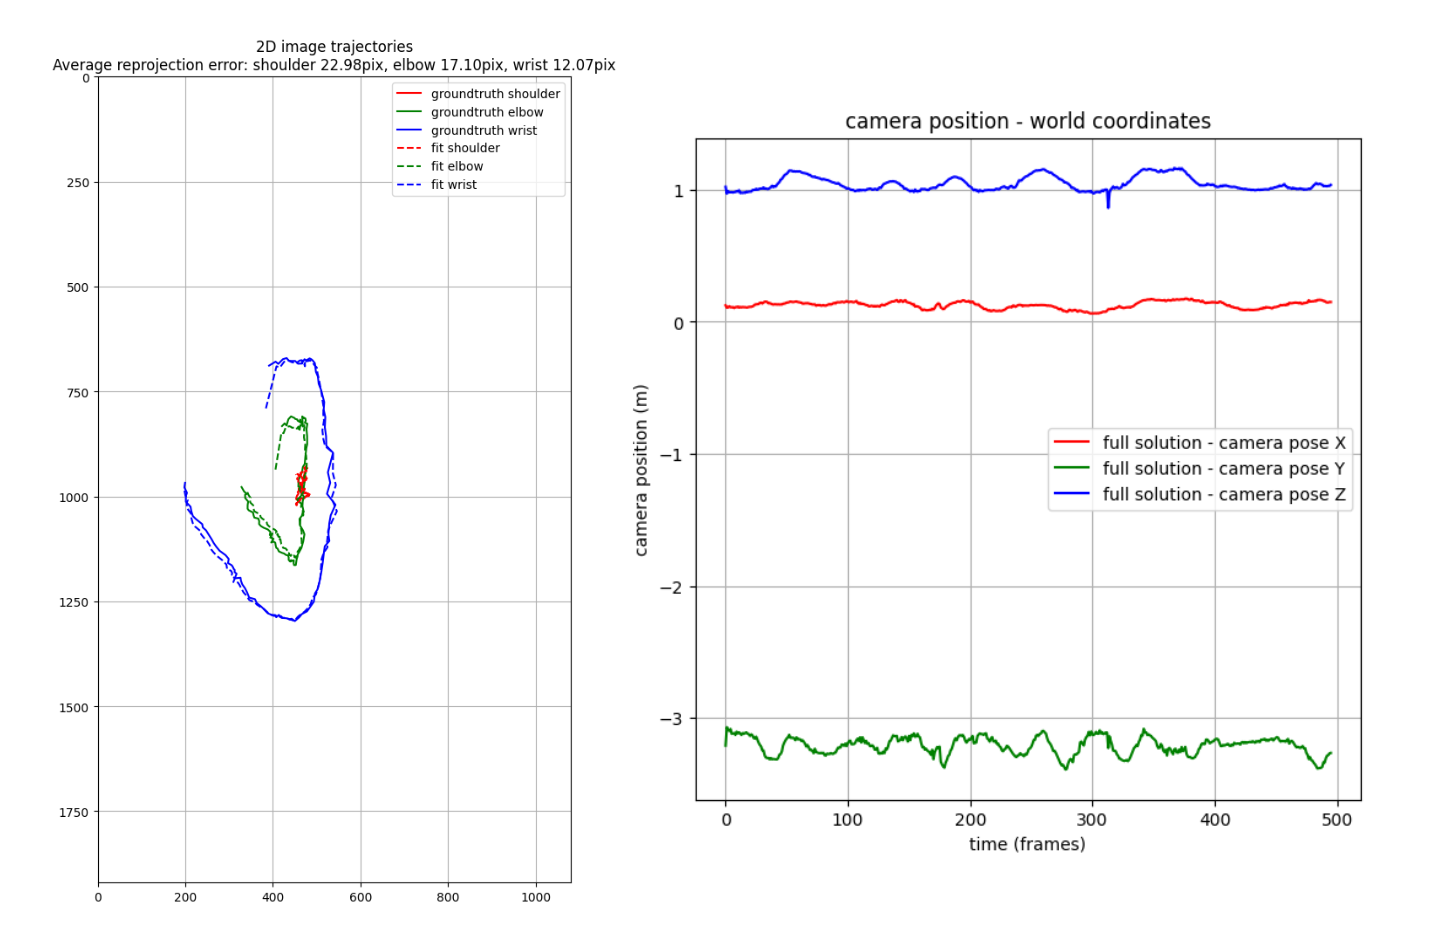
\includegraphics[width=8cm]{figures/camera_pose_fitting_collage.png}
    \caption{Left: projected arm 3D points onto the sensor after camera pose fitting - on the first 100 frames of the video (motion doing a circle with the arm). Average reprojection error reported here are computed on the 3 arm joints over the whole video.
    Right: Estimated distance from the camera to the shoulder is 3 meters wich is faithful to the real distance.}
    \label{fig:camera_fitting}
\end{figure}

\begin{figure*}
    \centering
    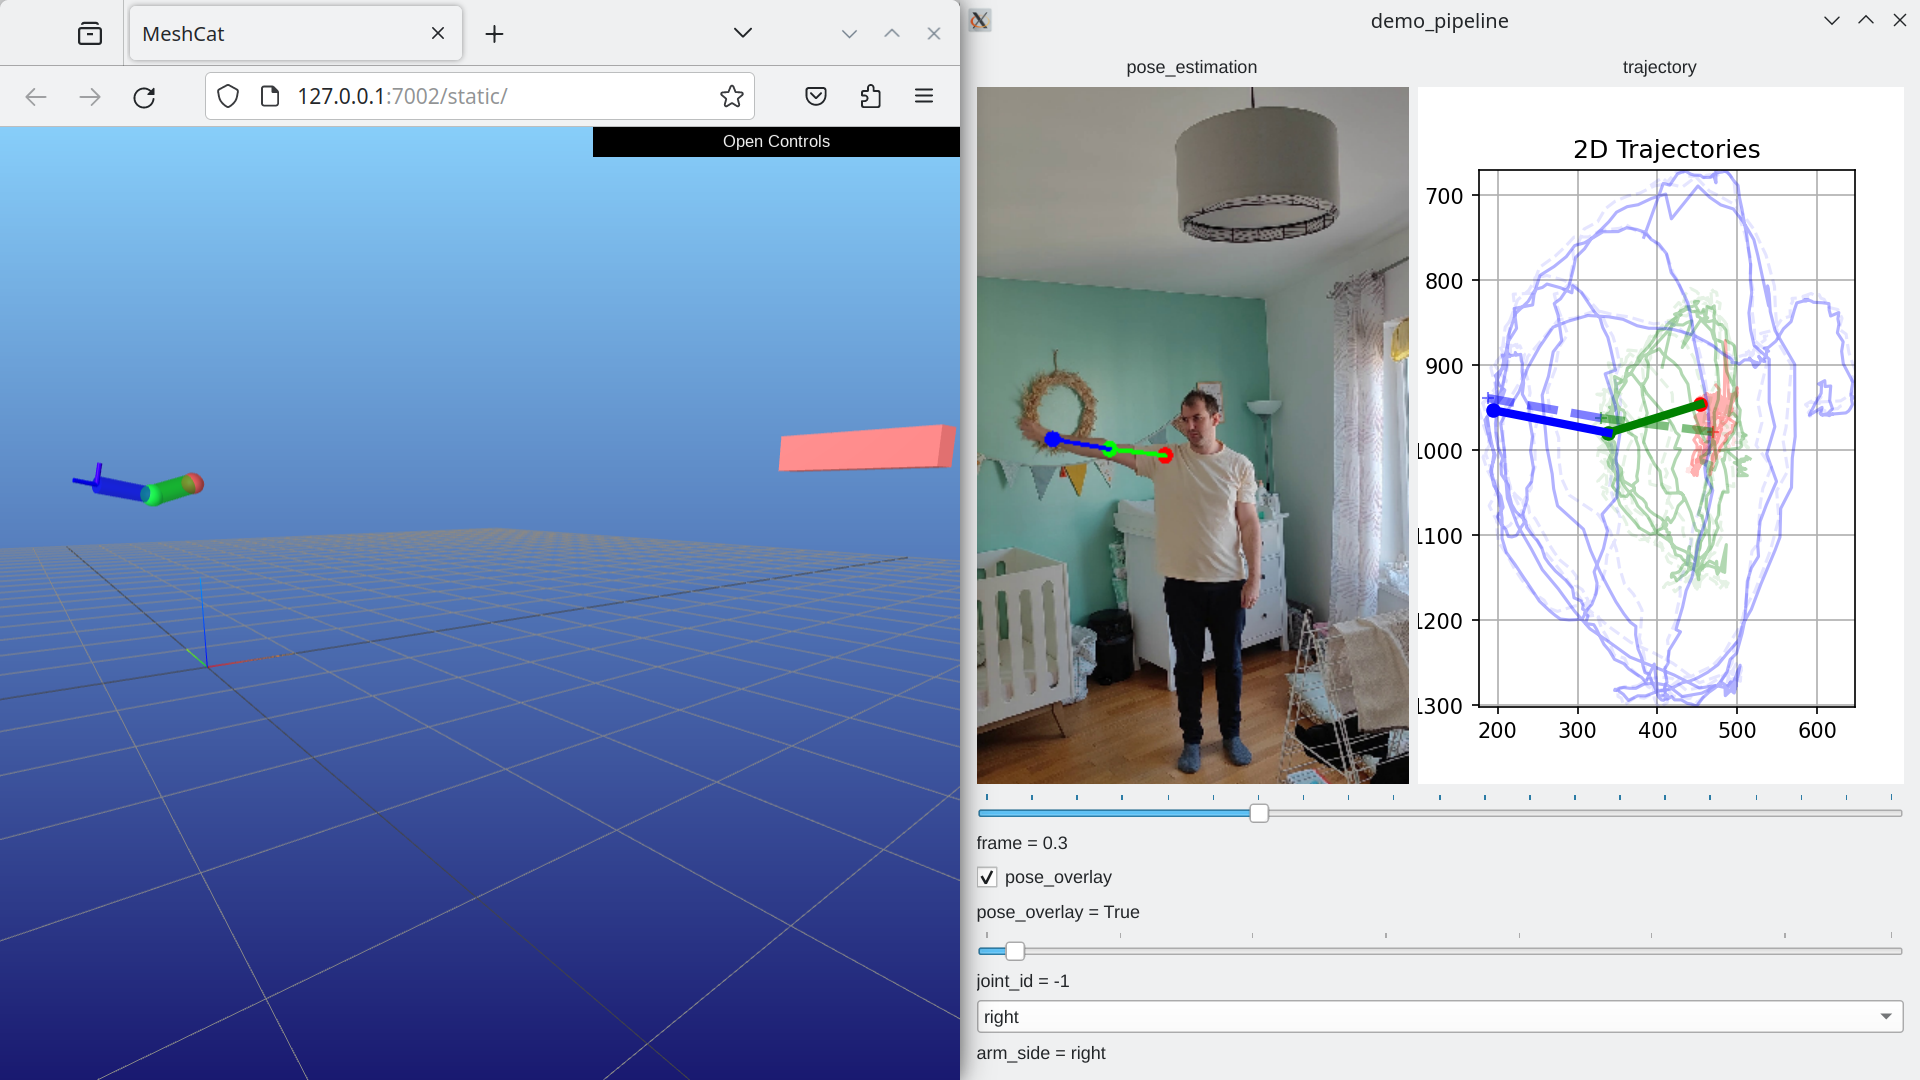
\includegraphics[width=16cm]{figures/arm_demo.png}
    \caption{Demo of the pose estimation pipeline.
    Left: Digital twin of the arm is synchronized witht the GUI. Camera is indicated in pink.
    Right: graphical user interface to select a specific frame
    and visualize the 2D joints position (dashed - right curve) aswell as the 3D reprojection of the arm (plain - right curve).}
    \label{fig:demo}
\end{figure*}

\subsection{Inverse dynamics optimizer}
\label{subsec:inverse_dynamics}

Given the simplifications discussed in~\cref{subsec:arm_model}, we reformulated the optimization problem as follows:

\begin{equation*}
    \begin{aligned}
        & \underset{q,\tau_m}{\text{minimize}} \quad \int_{0}^{T} l(q, \tau_m)\, dt \\
        & \text{subject to} \quad \dot{q} = f(q, \tau_m) \quad \text{(full-arm dynamics)}.
    \end{aligned}
\end{equation*}

\noindent\textbf{Variables.} The model variables consist of the arm's configuration vector \(q\) and the muscle joint torques \(\tau_m\). 
We adopted the midpoint method to approximate \(\dot{q}\) for its enhanced precision and because it provides velocity information precisely 
at instant \(t\).
\[
    \dot{q}_t = (q_{t + 1} - q_{t - 1}) / 2\Delta t
\]
Acceleration was computed in a similar fashion.

\noindent\textbf{Loss Functions.} Our loss function \(l\) omits \(l_{2D}\) due to the already accurate 3D pose estimates and 
excludes the pose likelihood term since we target only the arm. The remaining terms include:

\begin{itemize}
    \item 
        \(l_{3D}\): Ensures 3D position estimates align with the MediaPipe references.
    \item
        \(l_{\text{torque}}^h\): A regularization term penalizing high muscle torque values to favor energy-efficient movements.
    \item 
        Motion smoothness: Terms penalizing rapid movements or accelerations.
\end{itemize}

\noindent\textbf{Constraints.} The arm dynamics are governed by the Lagrangian equation:

\[
M(q)\ddot{q} + b(q, \dot{q}) = g(q) + \tau
\].

\noindent\textbf{Implementation.} We discretized the continuous-time problem, 
and use the midpoint method for derivative approximation. 
Pinocchio facilitated the computation of kinematic and dynamic quantities. 
The optimization was carried out using the Levenberg-Marquardt algorithm implemented in the SciPy library, 
chosen for its ease of integration with our Python-based pipeline. 
Constraint enforcement was achieved by embedding them as penalty terms within the loss function.

\subsection{Inverse Dynamics Results}
\label{subsec:dynamic_results}

Our initial tests of the optimizer were conducted on simulated data, enabling us to assess its performance and fine-tune the loss weights.

\noindent\textbf{Free Fall, Simulated.} We began with a simple free-fall scenario. The arm's initial configuration was horizontal to the ground, with an elbow angle of 
\(\pi/4\) radians. This simulation was performed using the Runge–Kutta 2 method, and the resulting ground truth is depicted 
in~\cref{fig:gt_free_fall}.

\begin{figure}
    \centering
    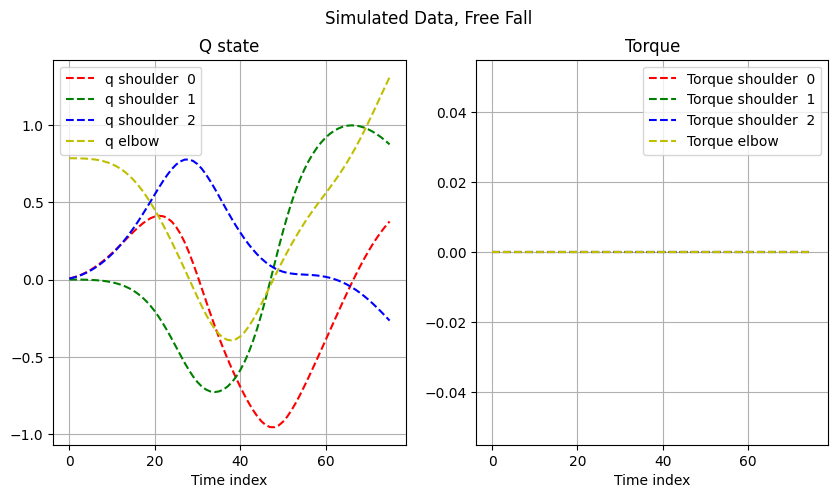
\includegraphics[width=8cm]{figures/free_fall_gt.png}
    \caption{Simulated ground truth data of free fall.}
    \label{fig:gt_free_fall}
\end{figure}

The optimizer was provided with the ground truth 3D poses and initial state vectors \(q_1, \ldots, q_T\) and zero torques. Without torque 
regularization, the optimizer yielded physically implausible torque estimations, despite low pose error, as shown 
in~\cref{fig:free_fall_no_torque}.

\begin{figure}
    \centering
    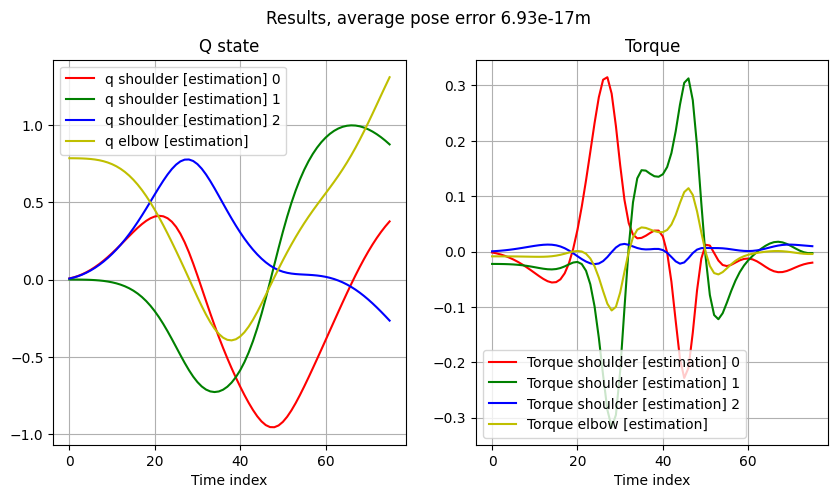
\includegraphics[width=8cm]{figures/free_fall_no_torque.png}
    \caption{Torque estimation without regularization, showing erroneous non-zero torques despite accurate pose estimation.}
    \label{fig:free_fall_no_torque}
\end{figure}

These inaccuracies are attributed to the midpoint approximation for velocities and accelerations, and potential undersampling, which 
introduces errors that the optimizer compensates for with non-zero torques.

Incorporating torque regularization significantly improved the results. While the pose error marginally increased, it remained within a 
reasonable range of a few millimeters. Crucially, the torque estimates were much closer to the expected zero value, as illustrated 
in~\cref{fig:free_fall_torque}.

\begin{figure}
    \centering
    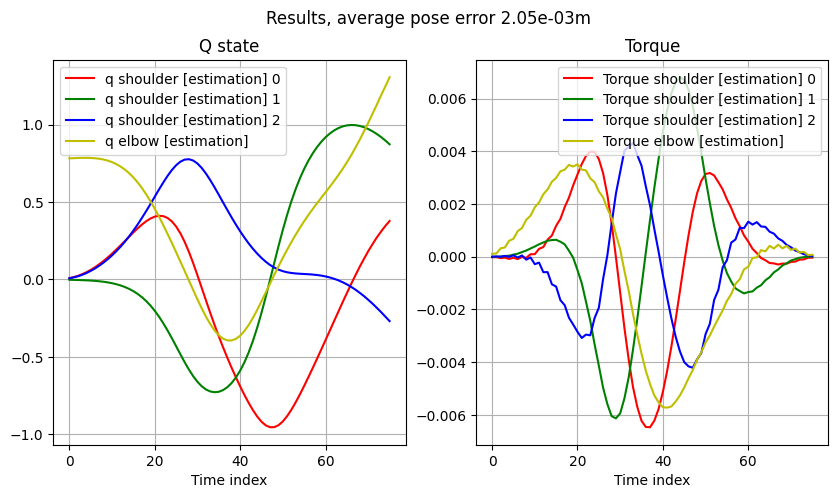
\includegraphics[width=8cm]{figures/free_fall_torque.png}
    \caption{Torque estimation with regularization, showing a pose error still fairly low and torques that align much more closely with the ground truth.}
    \label{fig:free_fall_torque}
\end{figure}

These findings highlight the importance of torque regularization in maintaining physical plausibility, especially when dealing with 
approximations issues.

\noindent\textbf{Free Fall with Friction, Simulated.} We tested the free fall with friction, represented by the equation 
\(\tau_m = -0.1\dot{q}\). This test aimed to evaluate the optimizer's ability to reconstruct non-trivial torque values. Ground truth and results, 
shown in~\cref{fig:free_fall_friction_gt} and~\cref{fig:free_fall_friction}, indicate that while the results are not flawless, 
they demonstrate the optimizer's capability to reconstruct coherent torques.

\begin{figure}
    \centering
    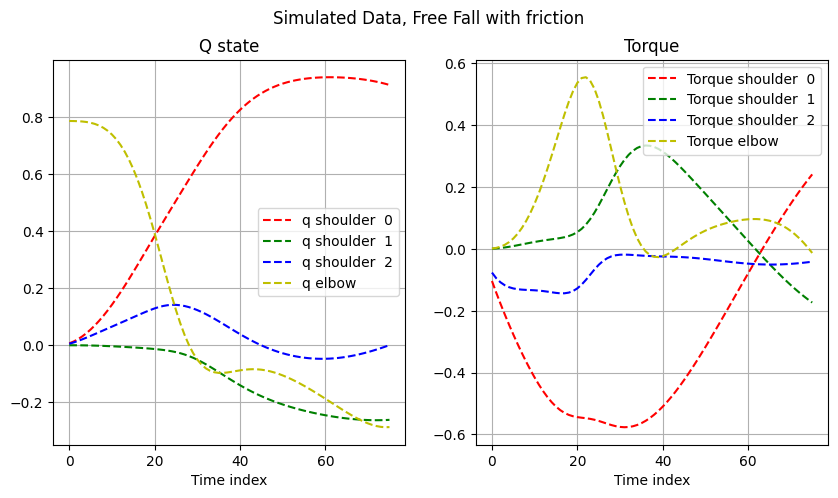
\includegraphics[width=8cm]{figures/free_fall_friction_gt.png}
    \caption{Simulated ground truth data of free fall with friction.}
    \label{fig:free_fall_friction_gt}
\end{figure}

\begin{figure}
    \centering
    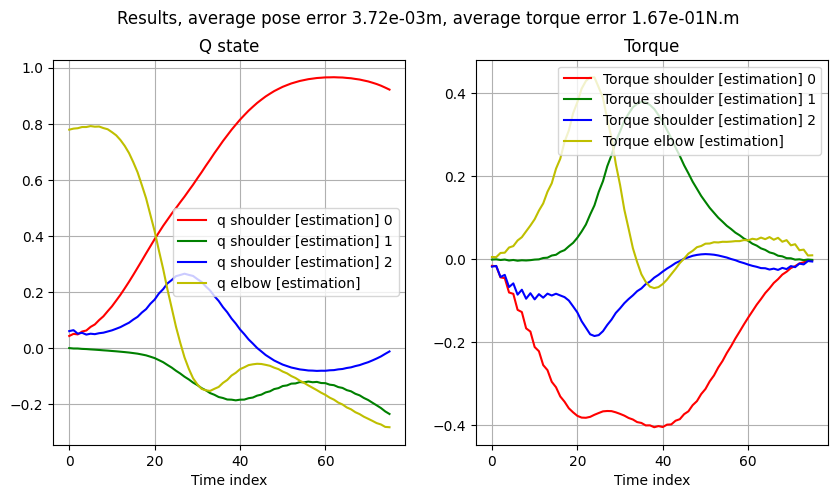
\includegraphics[width=8cm]{figures/free_fall_friction.png}
    \caption{Results of the optimization on the free fall with friction.}
    \label{fig:free_fall_friction}
\end{figure}


\noindent\textbf{Real Data.} When applying our optimizer to real-world data, we encountered several challenges. 
The optimization process in SciPy proved significantly slower on real data, with 2 seconds of video requiring upwards of 10 minutes of 
computation. Moreover, time constraints and the intricate nature of fine-tuning the loss weights for the optimizer prevented extensive 
testing on real data. Consequently, we could not obtain conclusive results from real-world experiments.